\chapter{Introduction}
\section{C$_4$ Photosynthesis \& C$_4$ rice}

\begin{wrapfigure}{r}{0.5\textwidth}%
	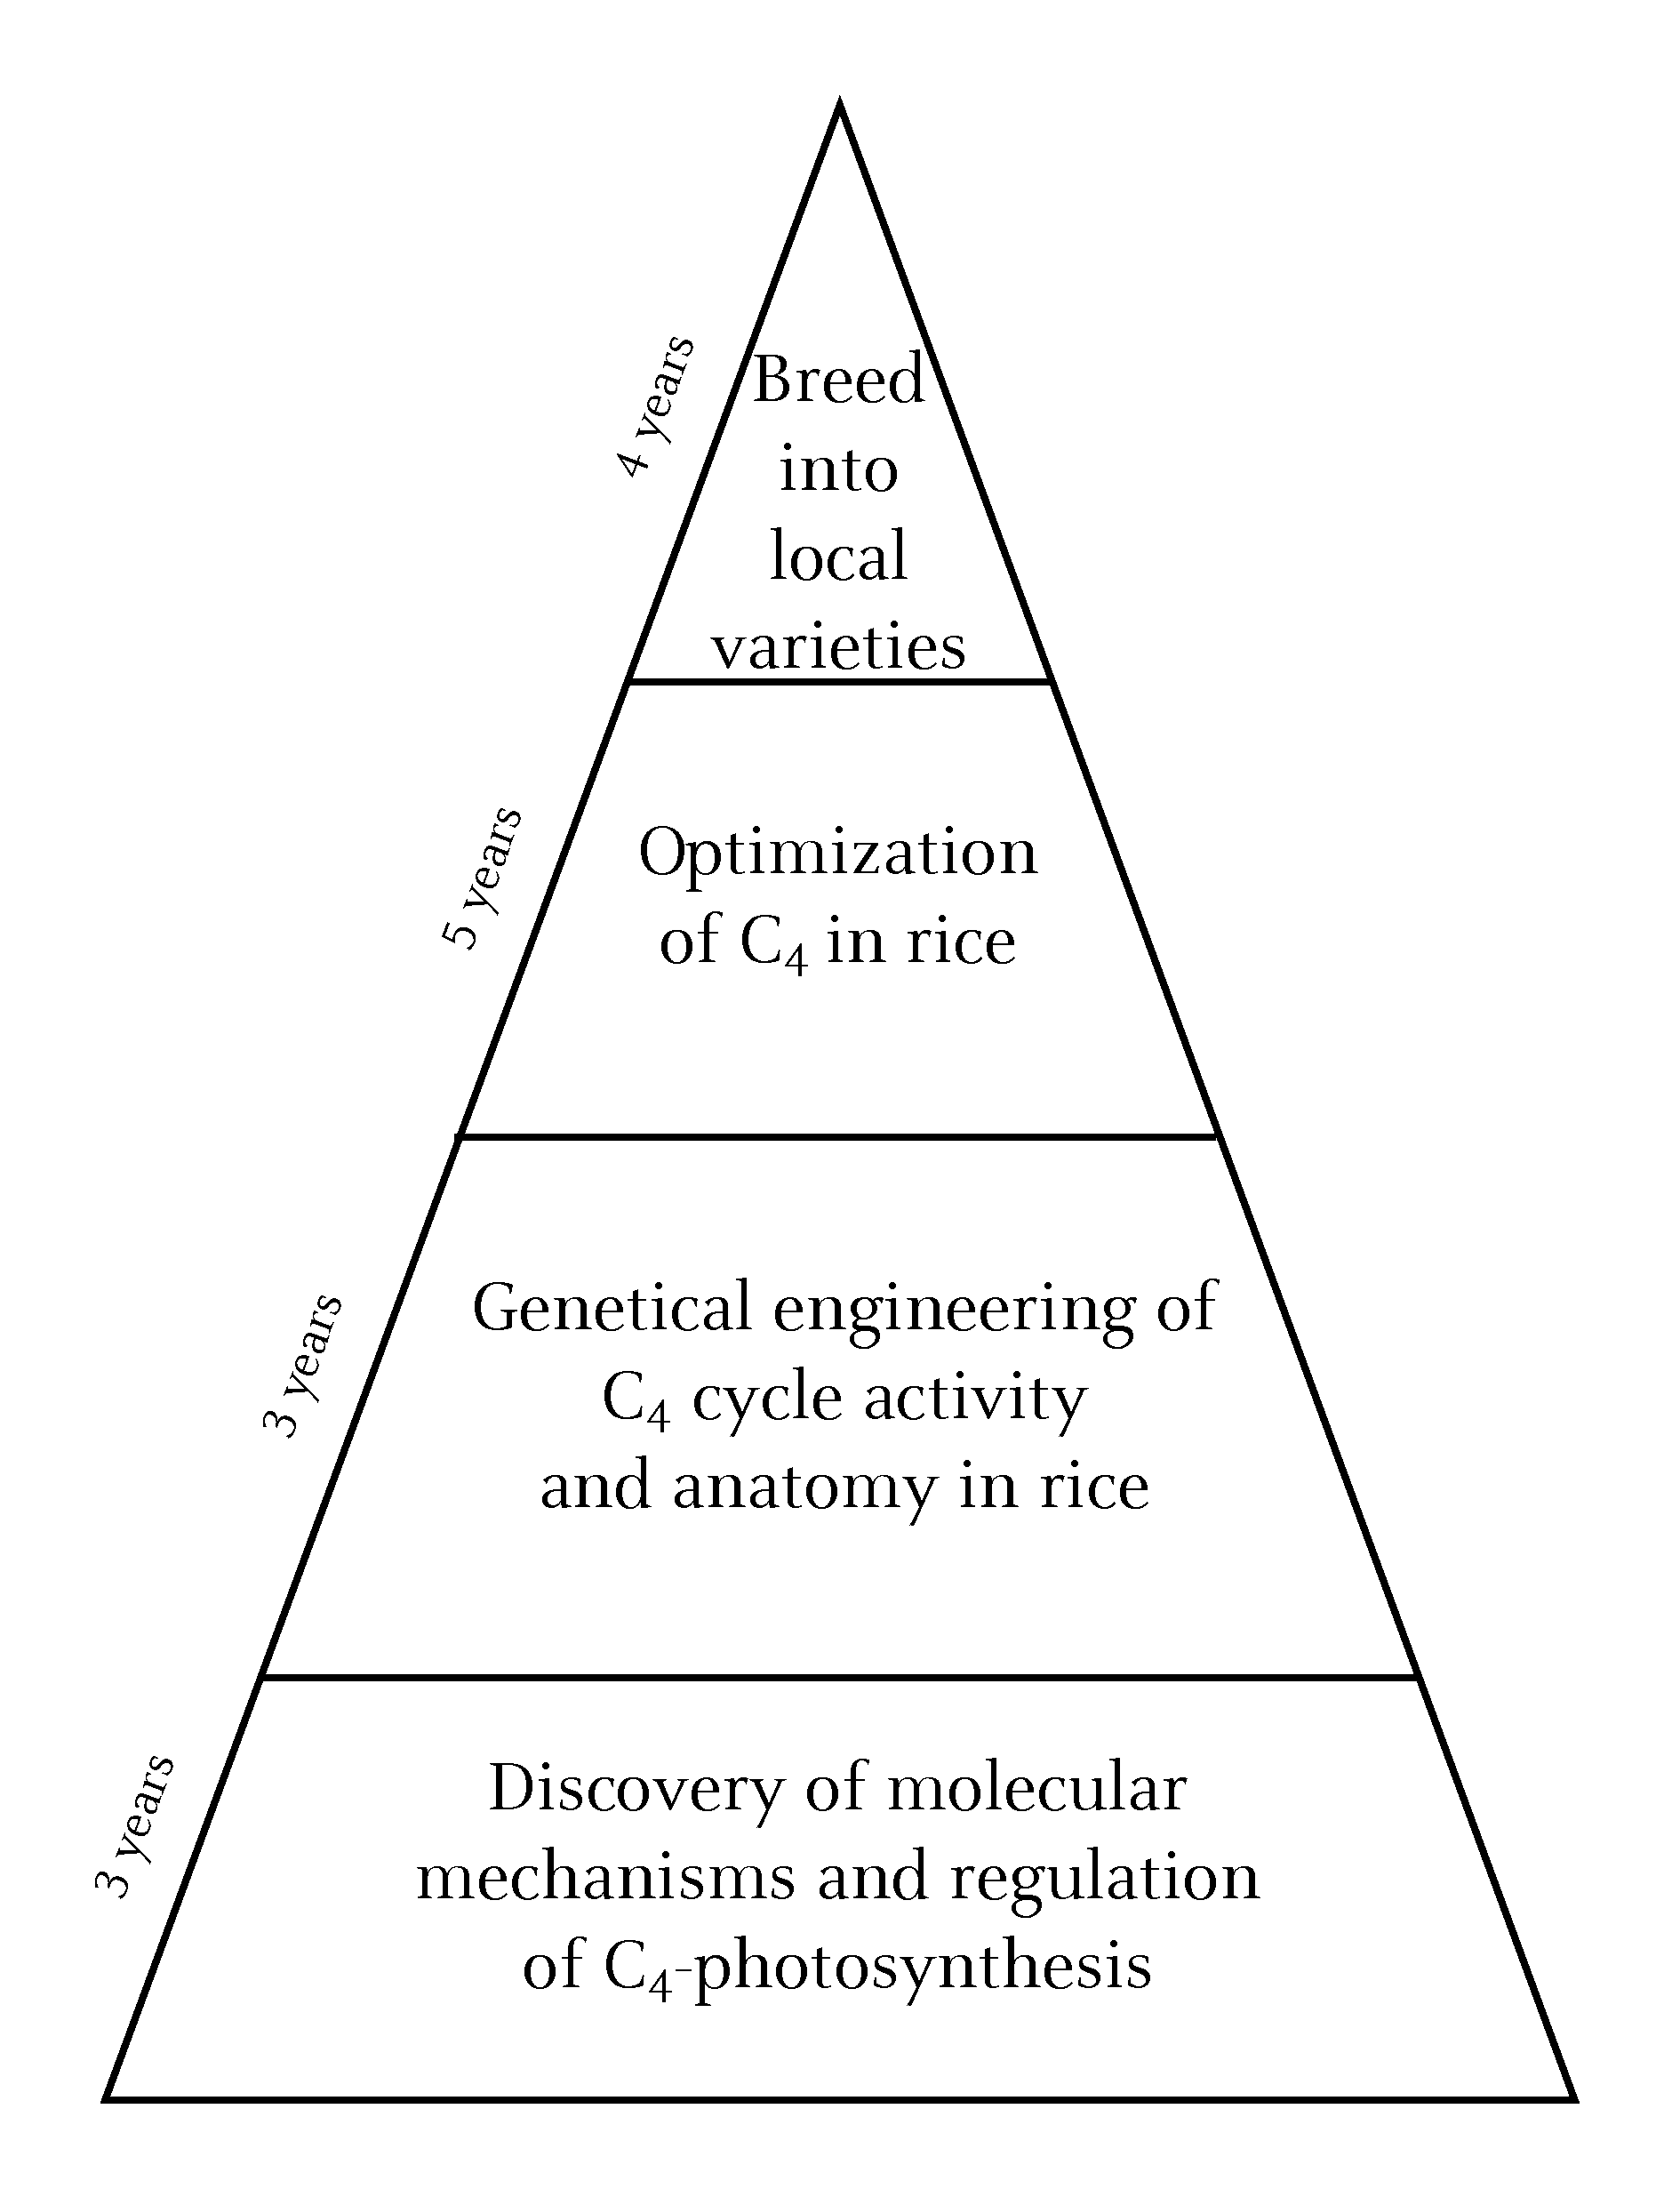
\includegraphics[width=0.48\textwidth]{images/C4_roadmap}%
	\caption{Roadmap for the C4-Rice Project \href{http://c4rice.irri.org}{(c4rice.irri.org)}}%
	\label{fig:c4rice_roadmap}%
\end{wrapfigure}

Around one billion people in the world feed on rice.
Rice is a cheap, non-perishable crop.
However, with growing population sizes the demand for rice increases, as well.
Now, C$_4$ photosynthesis is considered a very promising trait to cope with this demand by increasing yield.
\subsection{C$_3$ Photosynthesis}
Photosynthesis describes the conversion of CO$_2$ and light energy to sugars.
The primary fixation of CO2 is catalysed by RuBisCO.
CO$_2$ is attached to ribulose-1,5-bisphosphate (5C) yielding two molecules of phosphoglycerate (3C), hence the name C$_3$ photosynthesis.
However, a side reaction to RuBisCO fixing CO$_2$ is the fixation of oxygen.
The resulting molecule phosphoglycolate needs to be recycled at the loss of CO$_2$ and energy.
This process, called photorespiration reduces the overall efficiency.
Carbon fixation in plants performing only C$_3$ photosynthesis is, therefore, dependent on the CO$_2$ availability.
\subsection{C$_4$ photosynthesis}
C$_4$ photosynthesis is a trait that has evolved independently over 60 times throughout the plant kingdom.
Within the \species{Poaceae} (grasses) the evolutionary origins of C$_4$ photosynthesis are confined within the PACMAD clade.
Plants performing C$_4$ photosynthesis have evolved to avoid photorespiration and thus reduce energy loss.
The mechanism to avoid photorespiration consists of changes in metabolism as well as cell architecture.
A spatial separation of primary carbon fixation and fixation by RuBisCO has evolved by confining the expression of RuBisCO to the bundle sheath cells.
Primary CO$_2$ fixation then is catalysed by PEP carboxylase in the mesophyll cells.
The transfer of fixed CO$_2$ from mesophyll to bundle sheath is carried out by transfer acids, such as malate or aspartate.
After transfer to the bundle sheath, the fixed CO$_2$ is released again.
Thus the two step fixation of C$_4$ photosynthesis increases the CO$_2$ concentration in the vicinity of RuBisCO and suppresses the need for photorespiration.
As a consequence, less RuBisCO enzyme is needed.
Therefore, C$_4$ plants present a higher efficiency.
%More details wouldn't hurt
\subsection{C$_4$ rice}
While the demand for food is growing the area accessible to agriculture is shrinking.
One approach to induce a second green revolution is genetically engineering rice into a C$_4$ plant.
Expectations are not only that the yield will increase in current environments, but also rice will become accessible to more climate regions.
The International Rice Research Institute has laid out a roadmap to reach this goal.
In general, the project can be summarised as: Understand, Imitate, Optimise, and Breed.
That means, as depicted in figure \ref{fig:c4rice_roadmap}, they suggest a coordinated research effort over the next 15 years.
Starting with a detailed analysis of all molecular components involved in C$_4$.
Followed by engineering efforts to establish a C$_4$ like metabolism in rice.
Subsequently improving the cycle yield within rice transgenics.
Finally crossing rice transgenics with existing rice cultivars to generate location-adapted C$_4$ rice plants.
In terms of this roadmap, my work focuses on the analysis of the C$_4$-cycle within grasses.
It aims at describing a set of parts and interconnections in order to build a blueprint for re-engineering C$_4$ photosynthesis.
Thus the main driving force of my work was the question: 
\formatquote{Which transcripts are involved in creating the difference between C$_3$ and C$_4$ photosynthesis in two closely related grass species?}

%NOTES
Things I need to answer:
\begin{itemize}
	\item What is characteristic of C4-photosynthesis
	\item Why is it important to investigate
	\item What is the research goal
\end{itemize}
\section{Next-Generation Sequencing}
\section{Motivation}
